\documentclass[11pt]{article}

\usepackage{pablo}
\usepackage{tkz-tab}
\usepackage[a5paper,margin=0.5cm]{geometry}
\pagestyle{empty}

\begin{document}

\begin{center}
  \textsc{Trinômes} --- Révisions
\end{center}

\begin{exercice}[Fonction carrée]~
  \begin{enumerate}
    \item Calculer les valeurs exactes des carrés des nombres suivants :

      \begin{inparaenum}[(a)]
      \item $-3$
      \item $\frac{\sqrt{2}}{2}$
      \item $10^2$
      \item $\frac{3}{4}$
      \item $3\sqrt2$
      \end{inparaenum}.
    \item Ordonner, sans les calculer, les nombres suivants :
      \begin{inparaenum}[(a)]
      \item $26^2$ et $26,1^2$
      \item $(-4)^2$ et $(-5)^2$
      \item $(\sqrt{5}-1)^2$ et $(\sqrt{5}+1)^2$
      \item $3^2$ et $\pi^2$
      \item $(-\frac{1}{3})^2$ et $(-0,3)^2$
      \end{inparaenum}.
  \end{enumerate}
\end{exercice}

\begin{exercice}[Variations et extremums]
  Pour chacune des fonctions suivantes :
  \begin{enumerate}
    \item dresser son tableau de variations ;
    \item déterminer les coordonnées de son extremum ;
    \item tracer sa représentation graphique et vérifier graphiquement les réponses aux questions précédentes.
  \end{enumerate}
  \begin{inparaenum}[(a)]
  \item $2x^2-3x-1$ ;
  \item $-5x^2+2$ ;
  \item $3x^2$ ;
  \item $-x^2+6x+1$.
  \end{inparaenum}
\end{exercice}

\begin{exercice}[Forme canonique]~
  \begin{enumerate}
    \item
      \begin{enumerate}
        \item Montrer que $-(x-0,5)^2-3,75=-x^2+x-4$.
        \item En déduire les solutions de $-x^2+x-4=0$.
      \end{enumerate}
    \item Même question avec $(x+7)^2-9$ et $x^2+14x+40$.
    \item Même question avec $-3(x+\frac{1}{3})^2+9$ et $-3x^2+2x+\frac{26}{3}$.
  \end{enumerate}
\end{exercice}

\begin{exercice}[Géométrie]Le but de l'exercice est de trouver les points d'intersection du cercle $\cal C$ de centre $A(2,1)$ et de rayon 2 avec la droite d'équation $y=2x+1$. \emph{Les questions sont indépendantes.}
  \begin{enumerate}
    \item Faire une figure.
    \item Soit $M(x,y)$ un point du cercle. Calculer la distance $AM$ en fonction de $x$ et $y$, et montrer que $x^2-4x+y^2-2y+1=0$.
    \item En considérant l'équation de la droite $y=2x+1$, en déduire que $5x^2-4x=0$.
    \item Résoudre l'équation précédente pour trouver les valeurs possibles de $x$.
    \item En déduire les coordonnées des points d'intersection du cercle et de la droite.
  \end{enumerate}
\end{exercice}

\begin{exercice}[Problème]Exercice 14 p.118 du livre, corrigé à la fin du livre.
\end{exercice}

\newpage
\setcounter{exercice}{0}
\begin{exercice}[Fonction carrée]~
  \begin{enumerate}
    \item
      \begin{inparaenum}[(a)]
      \item $9$
      \item $\frac{1}{2}$
      \item $10^4$
      \item $\frac{9}{16}$
      \item $18$
      \end{inparaenum}.
    \item 
      \begin{inparaenum}[(a)]
      \item La fonction carrée est croissante pour les nombres positifs. $26<26,1$, donc $26^2<26,1^2$.\\
      \item La fonction carrée est décroissante pour les nombres négatifs. $-4>-5$, donc $(-4)^2<(-5)^2$.\\
      \item $(\sqrt{5}-1)^2<(\sqrt{5}+1)^2$
      \item $3^2<\pi^2$
      \item $(-\frac{1}{3})^2<(-0,3)^2$
      \end{inparaenum}
  \end{enumerate}
\end{exercice}

\begin{exercice}[Variations et extremums]
  \emph{Seul le cas de $2x^2-3x-1$ est corrigé. Pour les autres, tracer la fonction à la calculatrice pour vérifier vos résultats.}
  \begin{enumerate}
    \item Le nombre situé devant $x^2$ est positif, donc la fonction décroit puis croit. Son extremum est en $-\frac{b}{2a}=-\frac{-3}{2\times2}=\frac{3}{4}$. Le tableau est donc le suivant.

      \hfill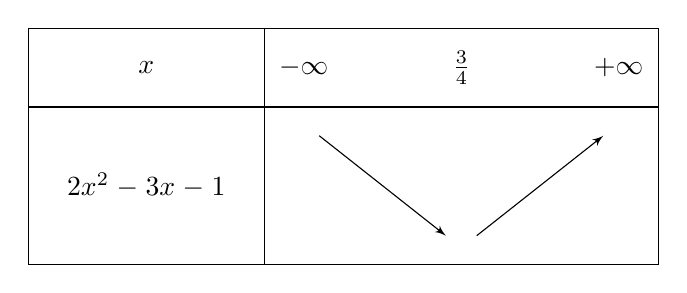
\begin{tikzpicture}
        \tkzTabInit[lgt=3,espcl=2]{$x$/1,$2x^2-3x-1$/2}%
        {$-\infty$,$\frac{3}{4}$,$+\infty$}%
        \tkzTabVar{+/ ,-/ ,+/}%
      \end{tikzpicture}
    \item Nous avons déjà calculé l'absisse de son extremum : $\frac{3}{4}$. Son ordonnée est $2\left(\frac{3}{4}\right)^2-3\frac{3}{4}-1=\ldots=-\frac{17}8$.
    \item \emph{Je vous laisse vérifier à la calculatrice.}
  \end{enumerate}
\end{exercice}

\begin{exercice}[Forme canonique]\emph{Seule la première question est corrigée}.
  \begin{enumerate}[(a)]
    \item \emph{Il suffit de développer la forme canonique.}
    \item Nous avons démontré que $-(x-0,5)^2-3,75=-x^2+x-4$. Donc 
    $-x^2+x-4=0$ est équivalent à $-(x-0,5)^2-3,75=0$ :

    $-(x-0,5)^2=3,75$

    $(x-0,5)^2=-3,75$

    Or un carré est toujours positif, donc cette équation n'a pas de solutions.
  \end{enumerate}
\end{exercice}

\begin{exercice}[Géométrie]\emph{Seuls des indices sont donnés.}
  \begin{enumerate}
      \setcounter{enumi}{1}
    \item Utiliser la formule permettant de calculer la longueur d'un segment : $AM=\sqrt{(x_M-x_A)^2+(y_M-y_A)^2}$, et remplacer les inconnues par les valeurs données dans l'énoncé.
    \item Utiliser la formule précédente, et remplacer $y$ par $2x+1$. Développer et réduire le résultat.
    \item Il y a une factorisation évidente en $x$. Ensuite, c'est une équation produit.
    \item Nous venons de calculer les valeurs de $x$. Utiliser l'équation de la droite pour calculer les valeurs de $y$ correspondantes.
  \end{enumerate}
\end{exercice}

\end{document}

